\documentclass[11pt,a4paper]{article}
%%%----------------------------------------------------------------------------%%%
%%%----------------------------------------------------------------------------%%%
%%% 
%%% ### Packages 
%%%
%%%----------------------------------------------------------------------------%%%
%%%----------------------------------------------------------------------------%%%
\usepackage{amsmath, amsthm, amssymb, nccbbb, bm, dsfont, pifont, fontawesome, graphicx, varioref, enumitem, mathtools, listings, xcolor, cite, fancyhdr, lastpage, lscape, subfig, graphicx, float, tabularx, algpseudocode, algorithm}

\RequirePackage[round,authoryear]{natbib}
\RequirePackage[colorlinks,citecolor=blue,urlcolor=blue]{hyperref}
\usepackage[cal=boondox]{mathalfa}
%\usepackage[numbers]{natbib}
\setlength{\topmargin}{-0.5in}
\setlength{\textheight}{10in}
\setlength{\oddsidemargin}{-.6in}
\setlength{\textwidth}{7.5in}
\hypersetup{colorlinks=true, linkcolor=blue, citecolor=red, urlcolor=blue}

%%%----------------------------------------------------------------------------%%%
%%%----------------------------------------------------------------------------%%%
%%% 
%%% ### Code 
%%%
%%%----------------------------------------------------------------------------%%%
%%%----------------------------------------------------------------------------%%%
\usepackage{listings}
\lstset{escapeinside=| |}
\usepackage[usenames,dvipsnames]{color}  
\definecolor{mygray}{rgb}{0.99,0.99,0.99}
\definecolor{myblue}{rgb}{0.0, 0.23, 0.63}
\definecolor{myred}{rgb}{0.75, 0.0, 0.0}
\definecolor{mygreen}{rgb}{0.4, 0.69, 0.2}  
\lstnewenvironment{R}{\lstset{ 
  language=R,
  basicstyle=\footnotesize\ttfamily, 
  numbers=left,
  numberstyle=\tiny\color{black},
  stepnumber=1,
  numbersep=5pt,
  backgroundcolor=\color{mygray},
  showspaces=false, 
  showstringspaces=false,
  showtabs=false, 
  frame=single,  
  rulecolor=\color{black},
  tabsize=4,
  captionpos=b,
  breaklines=true,
  breakatwhitespace=false,
  keywordstyle=\ttfamily\bfseries\color{myblue},
  commentstyle=\ttfamily\bfseries\color{myred},
  stringstyle=\ttfamily\bfseries\color{mygreen}
} 
}{}

%New colors defined below
\definecolor{codegreen}{rgb}{0,0.6,0}
\definecolor{codegray}{rgb}{0.5,0.5,0.5}
\definecolor{codepurple}{rgb}{0.58,0,0.82}
\definecolor{backcolour}{rgb}{0.95,0.95,0.92}

%Code listing style named "mystyle"
\lstdefinestyle{mystyle}{
  backgroundcolor=\color{backcolour}, commentstyle=\color{codegreen},
  keywordstyle=\color{magenta},
  numberstyle=\tiny\color{codegray},
  stringstyle=\color{codepurple},
  basicstyle=\ttfamily\footnotesize,
  breakatwhitespace=false,         
  breaklines=true,                 
  captionpos=b,                    
  keepspaces=true,                 
  numbers=left,                    
  numbersep=5pt,                  
  showspaces=false,                
  showstringspaces=false,
  showtabs=false,                  
  tabsize=2
}

%"mystyle" code listing set
\lstset{style=mystyle}

%%%----------------------------------------------------------------------------%%%
%%%----------------------------------------------------------------------------%%%
%%% 
%%% ### Box
%%%
%%%----------------------------------------------------------------------------%%%
%%%----------------------------------------------------------------------------%%%
\usepackage{tcolorbox}
\tcbuselibrary{breakable}
\newtcolorbox{mybox}{colback=yellow!5!white, colframe=gray!60!black, breakable}
\newtcolorbox{mybox0}{colback=white, colframe=gray!60!black, breakable}
	

%%%----------------------------------------------------------------------------%%%
%%%----------------------------------------------------------------------------%%%
%%% 
%%% ### Theorem style structures 
%%%
%%%----------------------------------------------------------------------------%%%
%%%----------------------------------------------------------------------------%%%
\numberwithin{equation}{section}
\theoremstyle{plain}
\newtheorem{theorem}{Theorem}[section]
\newtheorem{lemma}[theorem]{Lemma}
\newtheorem{corollary}[theorem]{Corollary}
\newtheorem{proposition}[theorem]{Proposition}
\newtheorem{condition}{Condition}[section]
\newtheorem{definition}{Definition}[section]
\theoremstyle{definition}
\newtheorem{example}{Example}[section]
\newtheorem{exercise}{Exercise}[section]
\newtheorem{remark}{Remark}[section]
\newtheorem{remark0}{Remark}
\newtheorem{question}{Question}


%%%----------------------------------------------------------------------------%%%
%%%----------------------------------------------------------------------------%%%
%%% 
%%% ### Operators 
%%%
%%%----------------------------------------------------------------------------%%%
%%%----------------------------------------------------------------------------%%%
\newcommand{\pr}{\mathsf{P}} 
\newcommand{\E}{\mathsf{E}} 
\newcommand{\median}{\mathop{\mathsf{median}}}
\newcommand{\Cov}{{\mathsf{Cov}}} 
\newcommand{\Corr}{{\mathsf{Corr}}} 
\newcommand{\Var}{{\mathsf{Var}}}
\newcommand{\SD}{{\mathsf{SD}}}
\newcommand{\CV}{{\mathsf{CV}}}
\newcommand{\Bias}{{\mathsf{Bias}}}
\newcommand{\AMSE}{\operatorname{\mathsf{AMSE}}}
\newcommand{\MSE}{\operatorname{\mathsf{MSE}}}
\newcommand{\ARE}{\mathsf{ARE}}
\newcommand{\AV}{\mathsf{AV}}
\newcommand{\CRLB}{{\mathsf{CRLB}}}

\newcommand{\pCorr}{\text{P}}
\newcommand{\sCorr}{\text{S}}
\newcommand{\kCorr}{\text{K}}
\newcommand{\bdCorr}{\text{BD}}
\newcommand{\cCorr}{\text{C}}


\newcommand{\inD}{    \overset{ \textnormal{d}   }{\rightarrow} }
\newcommand{\inAS}{   \overset{ \textnormal{a.s.}   }{\rightarrow} }
\newcommand{\inP}{    \overset{ \textnormal{pr}    }{\rightarrow} }
\newcommand{\inLp}{   \overset{ \mathcal{L}^p }{\rightarrow} }
\newcommand{\inMSE}{  \overset{ \textnormal{qm} }{\rightarrow} }
\newcommand{\inQM}{   \overset{ \textnormal{qm} }{\rightarrow} }
\newcommand{\indep}{\protect\mathpalette{\protect\independenT}{\perp}}
\def\independenT#1#2{\mathrel{\rlap{$#1#2$}\mkern4mu{#1#2}}}
\newcommand{\iid}{\textsc{iid}} 
\newcommand{\simIID}{   \overset{ \iid   }{\sim} }
\newcommand{\simIND}{   \overset{ {\indep}   }{\sim} }


\newcommand{\Bern}{\textnormal{Bern}} 
\newcommand{\Unif}{\textnormal{Unif}} 
\newcommand{\Normal}{\textnormal{N}} 
\newcommand{\logNormal}{\textnormal{LN}} 
\newcommand{\Bin}{\textnormal{Bin}} 
\newcommand{\NB}{\textnormal{NB}} 
\newcommand{\HG}{\textnormal{HG}} 
\newcommand{\Geom}{\textnormal{Geom}} 
\newcommand{\Beta }{\textnormal{Beta}} 
\newcommand{\BetaBin}{\textnormal{Beta-Bin}}
\newcommand{\Ga}{\textnormal{Ga}} 
\newcommand{\Exp}{\textnormal{Exp}} 
\newcommand{\Expo}{\textnormal{Expo}} 
\newcommand{\Po}{\textnormal{Po}} 
\newcommand{\Multi}{\textnormal{Multi}} 
\newcommand{\student}{\textnormal{t}} 
\newcommand{\Cauchy}{\textnormal{Cauchy}} 
\newcommand{\Pareto}{\textnormal{Pareto}} 
\newcommand{\Laplace}{\textnormal{Laplace}} 
\newcommand{\Logistic}{\textnormal{Logistic}} 
\newcommand{\Dir}{\textnormal{Dir}} 
\newcommand{\DP}{\textnormal{DP}} 
\newcommand{\Inv}{\textnormal{Inv-}} 
\newcommand{\F}{\textnormal{F}} 
\newcommand{\sign}{\textnormal{sign}}
\newcommand{\rank}{\textnormal{rank}}


\newcommand{\RV}{\textsc{rv}}
\newcommand{\cdf}{\textsc{cdf}} 
\newcommand{\cgf}{\textsc{cgf}} 
\newcommand{\pdf}{\textsc{pdf}} 
\newcommand{\pmf}{\textsc{pmf}} 
\newcommand{\chf}{\textsc{chf}} 
\newcommand{\mgf}{\textsc{mgf}}
\newcommand{\EF}{\textsc{EF}}
\newcommand{\NEF}{\textsc{NEF}}
\newcommand{\MLE}{\textsc{mle}}
\newcommand{\MAP}{\textsc{MAP}}
\newcommand{\Med}{\textsc{Med}}
\newcommand{\MME}{\textsc{mme}}
\newcommand{\QME}{\textsc{qme}}
\newcommand{\UMVUE}{\textsc{umvue}}
\newcommand{\MPT}{\textsc{MPT}}
\newcommand{\UMPT}{\textsc{UMPT}}
\newcommand{\LRT}{\textsc{LRT}}


\newcommand{\diag}{\mathop{\mathrm{diag}}}
\newcommand{\tr}{\mathop{\mathrm{tr}}}
\newcommand{\T}{\mathop{\mathrm{T}}}
\DeclareMathOperator*{\argmin}{arg\,min}
\DeclareMathOperator*{\argmax}{arg\,max}
\DeclareMathOperator{\sgn}{sgn}
\DeclareMathOperator{\logit}{logit}
\DeclareMathOperator{\expit}{expit}
\newcommand{\dd}{\textnormal{d}}


\newcommand{\lva}{{\color{myred}\ding{73}\ding{73}\ding{73}}}
\newcommand{\lvb}{{\color{myred}\ding{72}\ding{73}\ding{73}}}
\newcommand{\lvc}{{\color{myred}\ding{72}\ding{72}\ding{73}}}
\newcommand{\lvd}{{\color{myred}\ding{72}\ding{72}\ding{72}}}
\newcommand{\optional}{\noindent{\color{myblue}\faScissors}}
\newcommand{\Solution}{\noindent{\color{myblue}{{\textsc{Solution}}:~$\Big.$}}}
\newcommand{\take}{\noindent{\color{myblue}\faPaperPlaneO~\underline{\bf Takeaway}:~$\Big.$}}

% widecheck 
\DeclareFontFamily{U}{mathx}{\hyphenchar\font45}
\DeclareFontShape{U}{mathx}{m}{n}{
      <5> <6> <7> <8> <9> <10>
      <10.95> <12> <14.4> <17.28> <20.74> <24.88>
      mathx10
      }{}
\DeclareSymbolFont{mathx}{U}{mathx}{m}{n}
\DeclareFontSubstitution{U}{mathx}{m}{n}
\DeclareMathAccent{\widecheck}{0}{mathx}{"71}
\DeclareMathAccent{\wideparen}{0}{mathx}{"75}

\def\cs#1{\texttt{\char`\\#1}}

% Customize header and footer
\pagestyle{fancy}
\fancyhf{}
\fancyhead[L]{2021-22 Semester 2}
\fancyhead[R]{STAT4012 Statistical Principles of Deep Learning with Business}
\fancyfoot[R]{Page \thepage\ of \pageref*{LastPage}}
\fancyfoot[L]{\nouppercase{\leftmark}}
\renewcommand{\headrulewidth}{0.4pt} % default is 0pt
\renewcommand{\footrulewidth}{0.4pt} % default is 0pt

\usepackage[bottom]{footmisc}

\newcounter{magicrownumbers}
\newcommand\rownumber{\stepcounter{magicrownumbers}\arabic{magicrownumbers}}

\usepackage[table]{xcolor}
%------------------------------------------------------------------------------

\begin{document}
    
    % Page 0 for names and table of contents
    \thispagestyle{empty}
    \pagenumbering{gobble} 
    \title{\textsc{STAT 4012} -- Statistical Principles of Deep Learning with Business \\ Group Project}
    \author{
        KWOK Ho Hin (SID: \texttt{1155126159}) \\
        LAI Tsz Chun (SID: \texttt{1155125208}) \\
        LAM Wai Chiu (SID: \texttt{1155152095}) \\
        LAW Yiu Leung Eric (SID: \texttt{1155149315}) \\
        TSOI Tung Sing (SID: \texttt{1155127274}) \\
        LO Chak Kin Steven (SID: \texttt{1155125491})
    }
    \date{\today}
    \maketitle
    
    % \newpage
    \tableofcontents
    \thispagestyle{empty}
    \pagenumbering{gobble} 
    \thispagestyle{empty}
    \newpage
    
    % Section 1
    \pagenumbering{arabic}
    \setcounter{page}{1}
    
    % Emotion Detection
    \section{Real Time Emotion Detection Deep Learning Model}
    \textbf{This section is contributed by LAI Tsz Chun (SID: 1155125208), LAM Wai Chui (SID: 1155152095) and LAW Yiu Leung Eric (SID: 1155149315).}
    
    \subsection{Introduction}
    The study of Convolutional Neural Network (CNN) in this course has inspired us the importance of CNN in image classification. We further extend our inspiration to facial expression recognition. Emotion serves as an immediate means for humans to interact and sometimes it also affects human behavior. Hence, we aim to replicate human emotional recognition using CNN in a real time manner. \\
    \\
    We designed to build an artificial intelligence (AI) that consists of two models. The first model is a face detection model borrowed from MTCNN. The second model is our custom CNN model for facial expression recognition. The main objective is to recognize seven basic emotional expressions (Angry, Disgust, Fear, Happy, Sad and Surprise, Neutral) by our custom model with a satisfactory accuracy rate. A demonstration using our model in real time and a model evaluation are also covered to see the performance of the model.

    
    \subsection{Dataset}
    \href{https://www.kaggle.com/datasets/msambare/fer2013}{FER-2013} \cite{FER2013} dataset from Kaggle is selected for model training. The data consists of $48 \times 48$ pixel grayscale images of faces. The faces have been automatically registered so that the face is more or less centred and occupies about the same amount of space in each image. The faces are categorized into seven categories (0=Angry, 1=Disgust, 2=Fear, 3=Happy, 4=Neutral, 5=Sad, 6=Surprise). The training set consists of 28,709 examples and the public test set consists of 3,589 examples. 
    \begin{figure}[H]
        \centering
        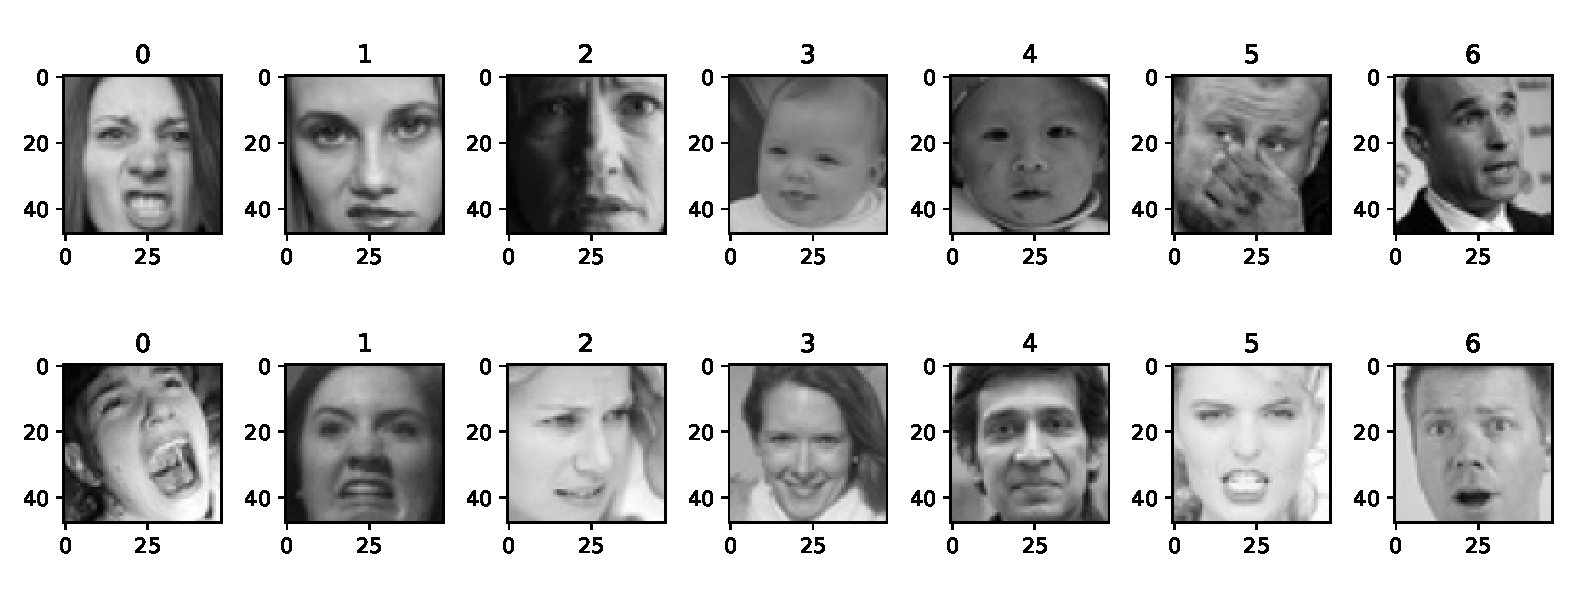
\includegraphics[width = 0.9\textwidth]{emotion_detection/plot/train.pdf}
        \caption{Training Dataset}
        \label{fig:train_dataset}
    \end{figure}
    \begin{figure}[H]
        \centering
        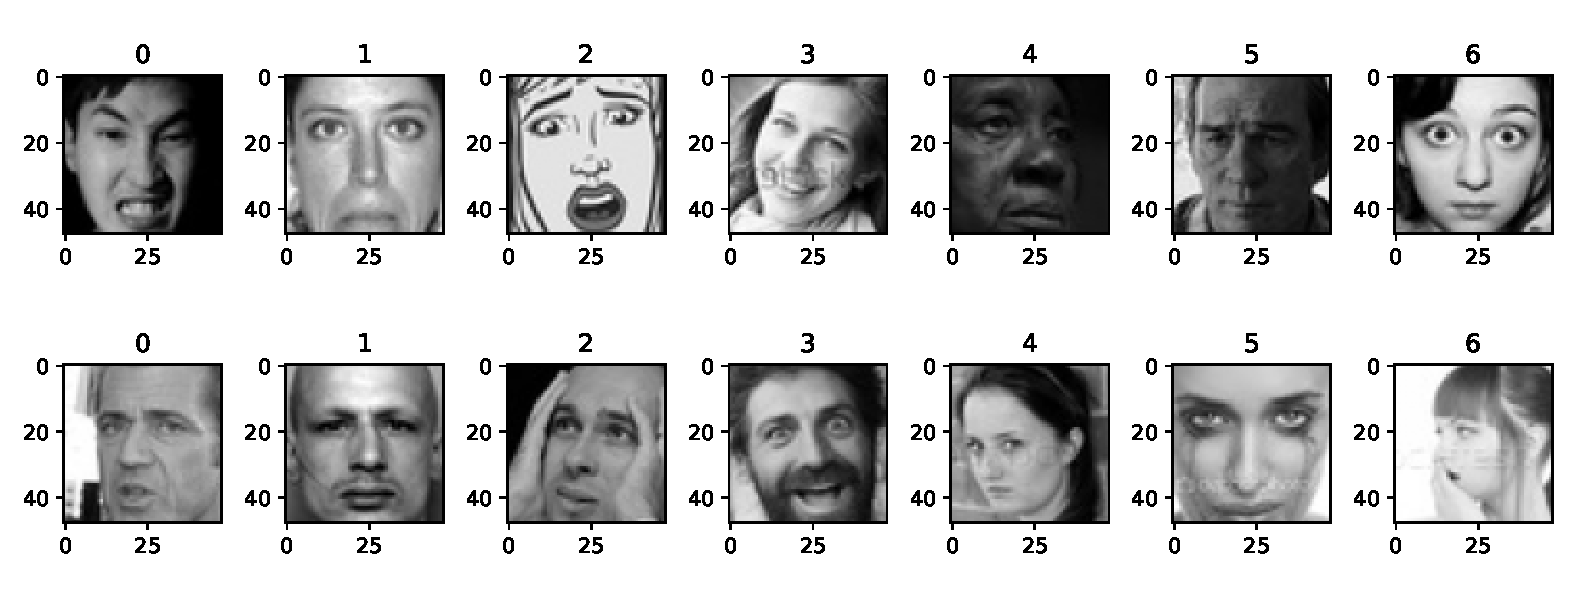
\includegraphics[width = 0.9\textwidth]{emotion_detection/plot/test.pdf}
        \caption{Testing Dataset}
        \label{fig:test_dataset}
    \end{figure}
    
    % \subsection{Project Description}
    
    \subsection{Data Preparation for Model Training}
    The data are stored in \texttt{.jpg} format, in order to use them, we must perform pre-processing to the dataset. We acknowledge that \texttt{Tensorflow} does provide a function \texttt{tf.keras.preprocessing.image.ImageDataGenerator}\footnote{\url{https://www.tensorflow.org/api_docs/python/tf/keras/preprocessing/image/ImageDataGenerator}} for loading image files from folders into data generator, which only load the image into tensor when in needed. However, we insist to save the data in \texttt{NumPy} format in order to speed up training process. Yet, this method have some drawbacks, which occupies about 2 GB of RAM for loading datasets before training, and extra storage space in hard disk.
    \begin{enumerate}
        \item Read the images using \texttt{OpenCV}.
        \item Normalized the grayscale from [0, 255] to [0, 1] for increasing training speed.
        \item Stack up 1-channel grayscale array into 3-channel RGB array, as the final use would be RGB pictures.
        \item Encode the labels.
        \item Save the array to \texttt{NumPy} array, then save as \texttt{Pickle} file.
    \end{enumerate}
    Noted that the dataset have already split into training and testing datasets from Kaggle, we do not need to split them. \\
    \\
    \textbf{Implementation:} \texttt{emotion\_detection\textbackslash src\textbackslash read\_data.ipynb}
        
    % \subsubsection{Create Numpy Array}
    
    % \subsubsection{Splitting Training Dataset and Testing Dataset}
    
    \subsection{Model Design}
    We intended to build a real-time emotion detection AI, so there are two separated models needed, namely face detection model and emotion detection model. Flow of the model:
    \begin{enumerate}
        \item Detect face(s) in a photo.
        \item Capture pixels of the face(s) and resize to $48 \times 48$.
        \item Classify emotion of the faces(s).
    \end{enumerate}
    
    % \newpage
    \subsubsection{MTCNN Face Detection Model}
    MTCNN is a python (pip) library written by Github user \href{https://github.com/ipazc/mtcnn}{ipacz} \cite{MTCNN}, which implements the paper by Zhang, Kaipeng et al. “Joint Face Detection and Alignment Using Multitask Cascaded Convolutional Networks.” \cite{1604.02878} In this paper, they propose a deep cascaded multi-task framework using different features of “sub-models” to each boost their correlating strengths. We choose MTCNN model for detecting faces in picture.
    \begin{figure}[H]
        \centering
        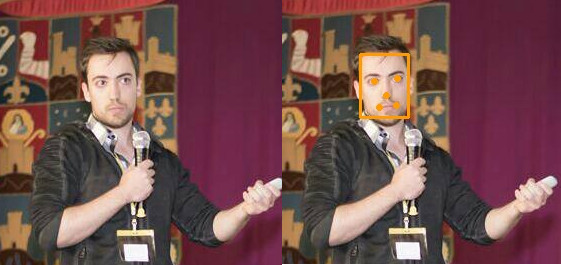
\includegraphics[width = 0.8\textwidth]{written_report/pictures/mtcnn.jpg}
        \caption{Face Detection using MTCNN}
        \label{fig:MTCNN}
    \end{figure}
    
    \subsubsection{Augmentation}
    Too avoid over fitting, we use a technique called augmentation to increase the diversity of your training set by applying random flip and slight rotation.
    \begin{figure}[H]
        \centering
        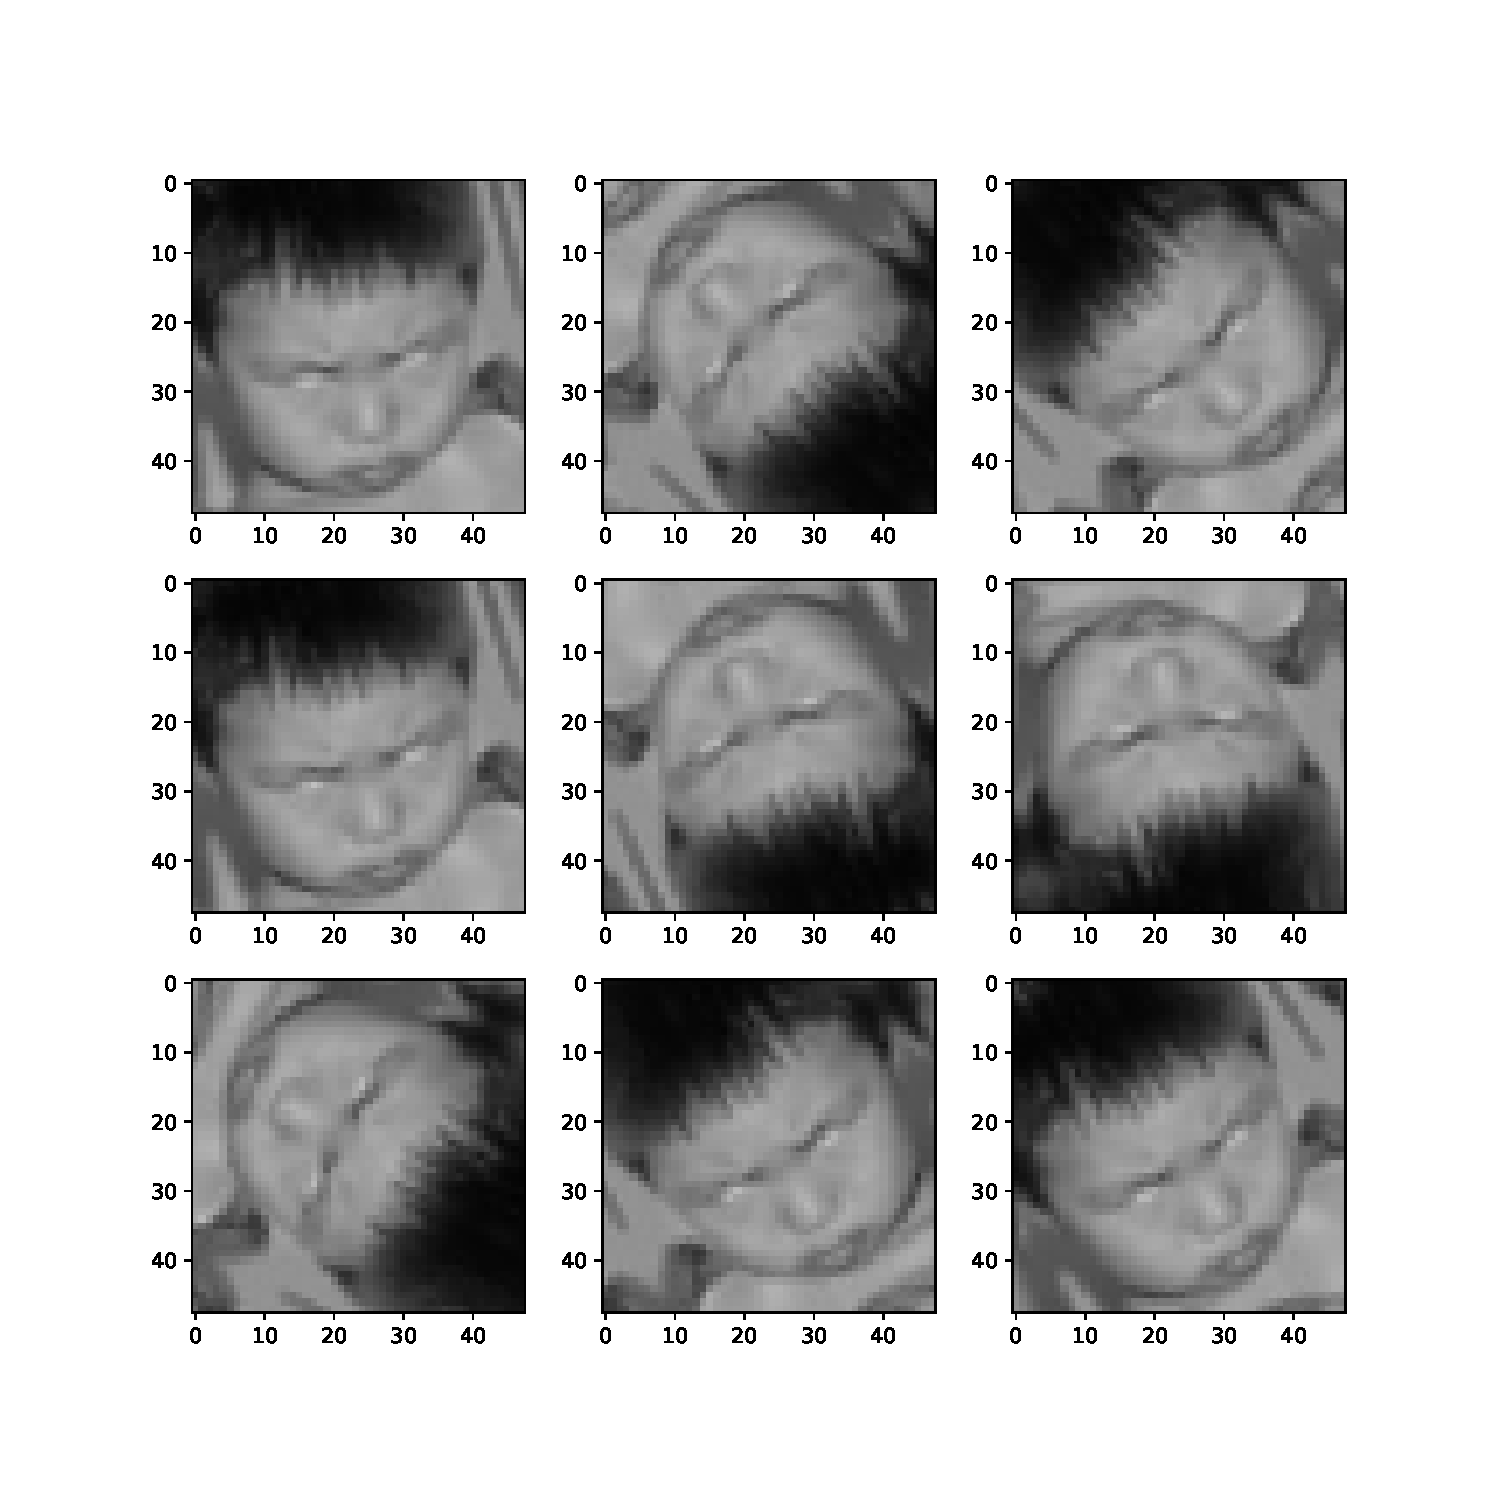
\includegraphics[width = 0.7\textwidth]{emotion_detection/plot/augmentation.pdf}
        \caption{Augmentation}
        \label{fig:augmentation}
    \end{figure}
    
    \subsubsection{Emotion Detection Model}
    We create and train a custom CNN model. After the augmentation function mentioned above, the pixels are passing through 5 blocks of convolution layers and 2 hidden fully-connected layers. All convolution layers and hidden layers  are using RELU activation, expect the output layer is using softmax activation. \\
    \\
    Block 1 and 2 each consists 2 layers of CNN layers, while block 3 to 5 each consists 3 layers of CNN layers, the filter size is increasing block by block from 64 to 512. In additions, each block has it own batch normalization layers, and from block 2 to 5, l2 regularization is used for kernel regularization. \\
    \\
    \textbf{Implementation:} \texttt{emotion\_detection\textbackslash src\textbackslash model\_train.ipynb}
    
    \subsubsection{Compile Model}
    The loss function is set to be sparse categorical cross-entropy, which is most suitable for multi-classes classification artificial neural network (ANN). Also, Adam is used as the optimizer for model training, with a common learning rate $\ng = 10^{-4}$. \\
    \\
    In total, this model consists 33,631,815 parameters, in which 33,628,871 of them are trainable and 2,944 are non-trainable (parameters for batch normalization).
    
    \begin{figure}[H]
        \centering
        \begin{minipage}[b]{.4\textwidth}
            \centering
            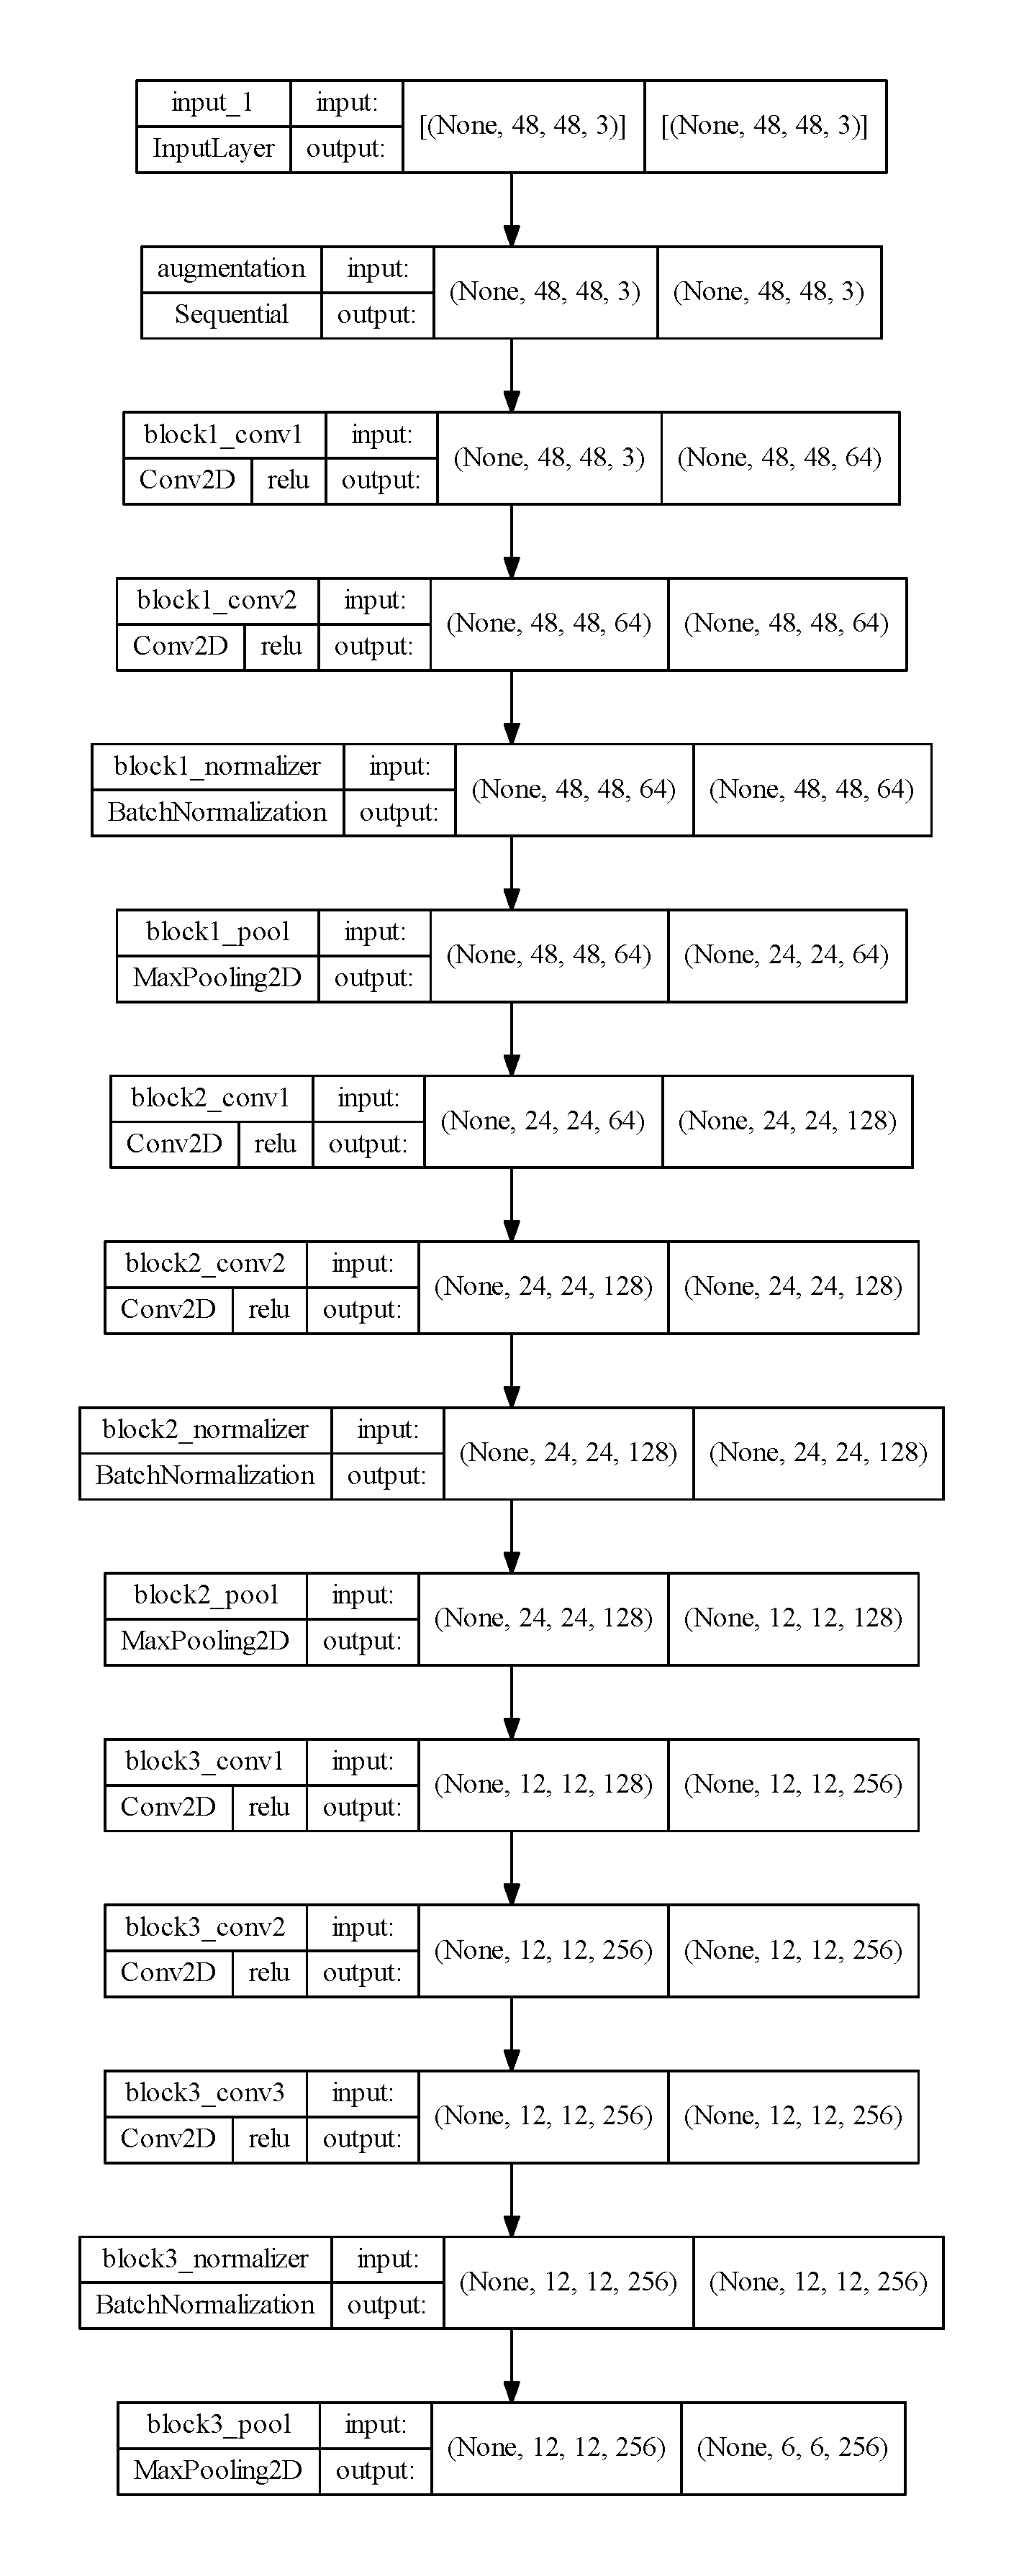
\includegraphics[height = 0.9\textheight]{written_report/pictures/model_1.pdf}
        \end{minipage}
        \begin{minipage}[b]{.4\textwidth}
            \centering
            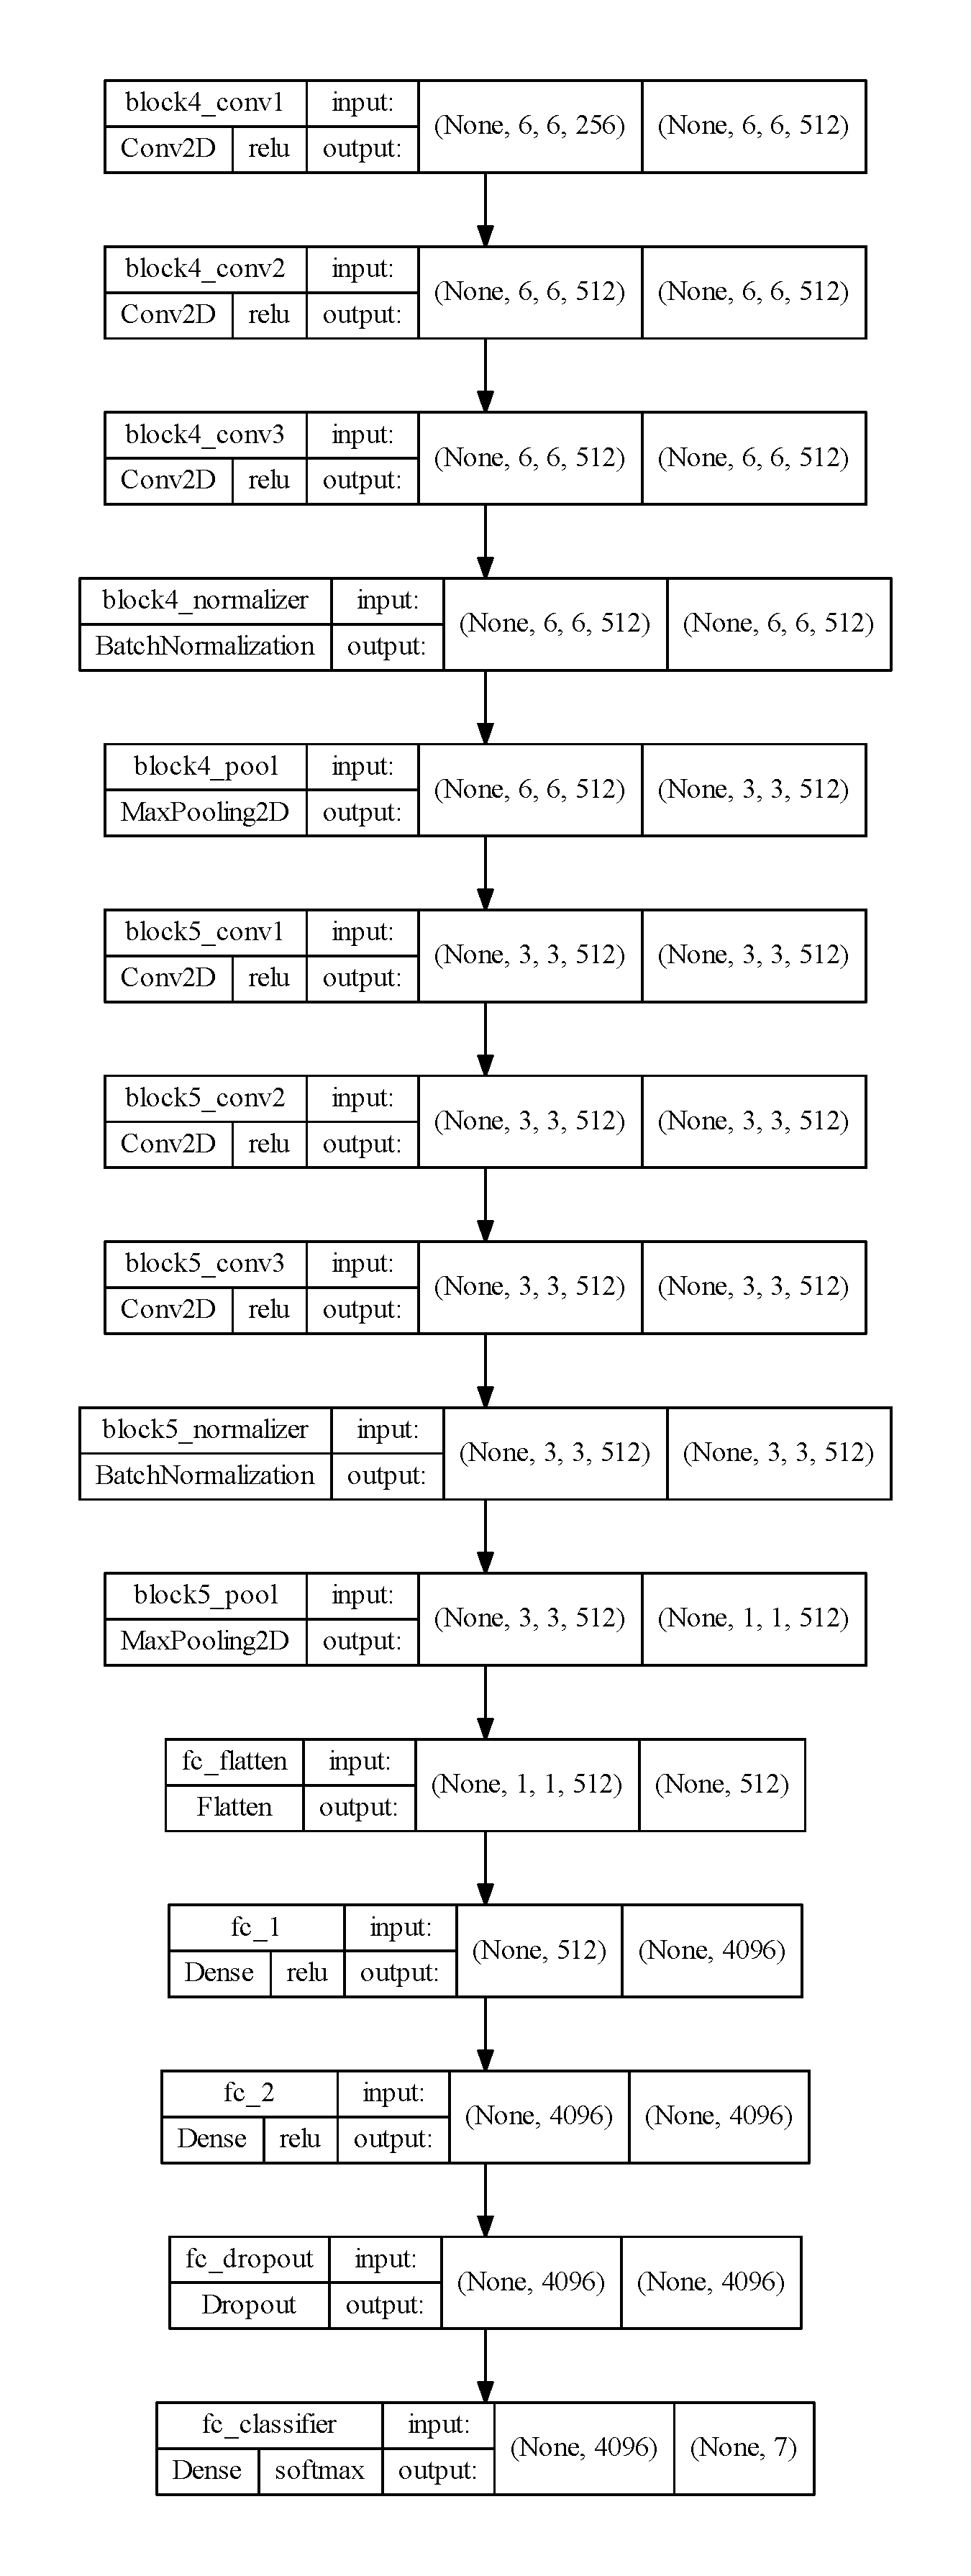
\includegraphics[height = 0.9\textheight]{written_report/pictures/model_2.pdf}
        \end{minipage}
        \caption{Model Architecture}
        \label{fig:model}
    \end{figure}
    
    \subsection{Model Training}
    \subsubsection{Training Specifications}
    We aim to train the model to an optimal point, neither overfiting nor underfitting. Thus, we set to train 200 epochs, but training procedure is expected to be stopped early, if the validation accuracy does not improve after 15 epochs. The final model would the one which has best validation accuracy. \\
    \\
    Training a very deep CNN requires huge amount of GPU power, in which non of our group member could afford it. Thanks to Google, they offer \href{https://research.google.com/colaboratory/}{Colab} which let us to use their GPU for free.
    
    \subsubsection{Model Evaluation}
    \begin{figure}[H]
        \centering
        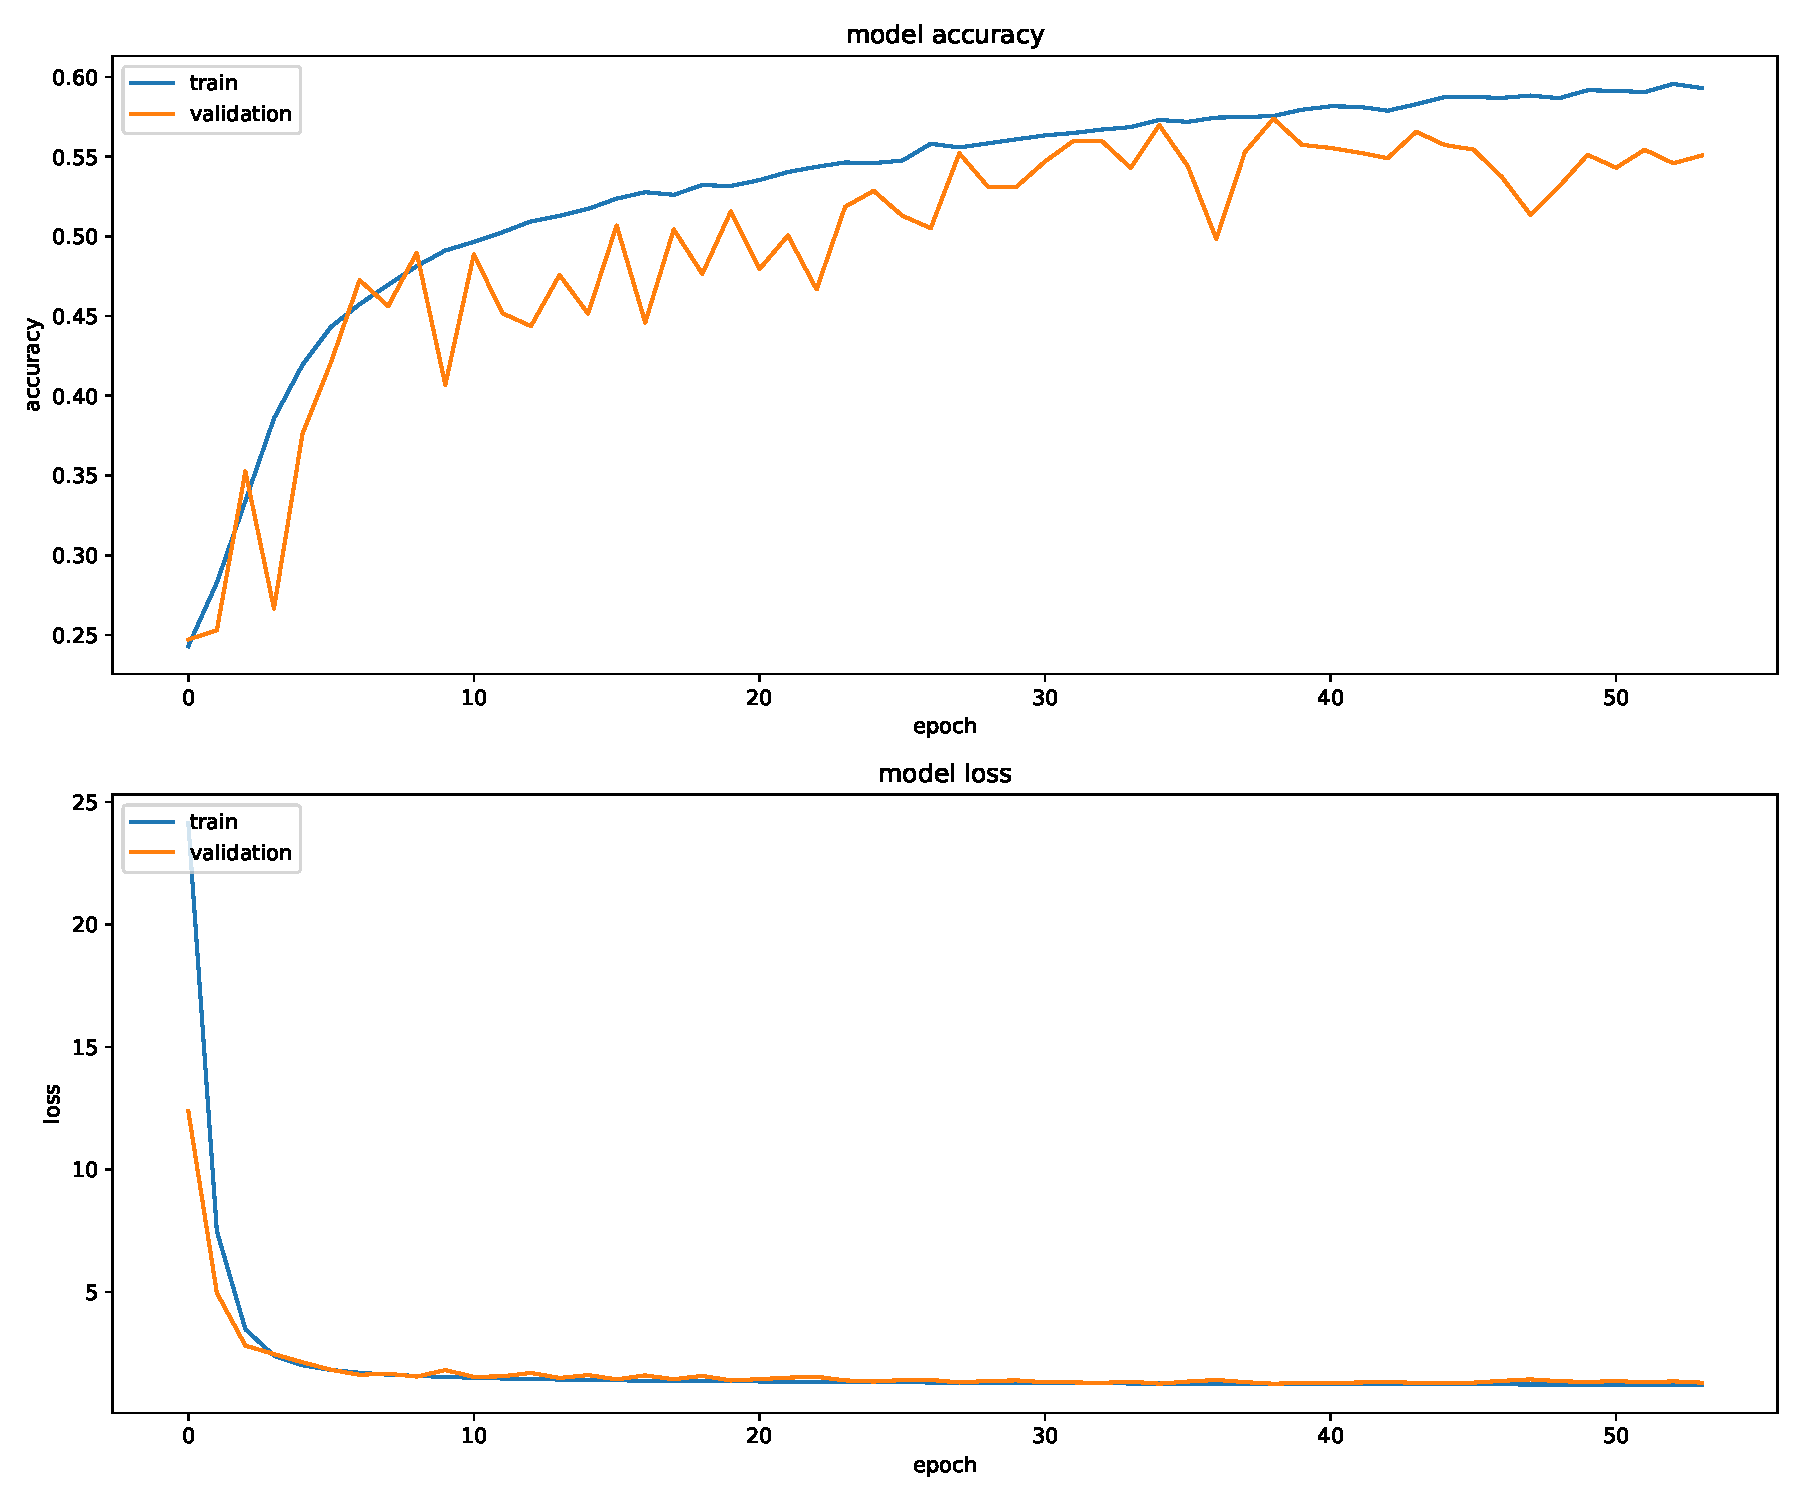
\includegraphics[width = 0.9\textwidth]{emotion_detection/plot/history.pdf}
        \caption{Loss and Accuracy}
        \label{fig:loss_acc}
    \end{figure}
    Early stopping was trigger after 54 epochs, the model eventually achieved valid accuracy at around 0.58. \\
    With a \href{https://www.nvidia.com/en-us/data-center/tesla-t4/}{Tesla T4}\footnote{Nvidia Tesla T4 is optimized for mainstream computing environments and features multi-precision Turing Tensor Cores and new RT Cores} GPU, each epoch requires around 70 seconds, in total around an hour for complete training, which is reasonable.
    
    \newpage
    \subsection{Demonstration}
    
    % \subsubsection{Import Video}
    This AI emotion detection solution not only support real time detection, it also allows end-users input a video for detection. For demonstration, we use a video clip from \href{https://www.youtube.com/watch?v=myjEoDypUD8&pbjreload=102}{94th Academy Awards}\footnote{the video clip is adjusted to 3 fps}. With sufficient resolutions, the AI could easily detect happy faces.
    \begin{figure}[H]
        \centering
        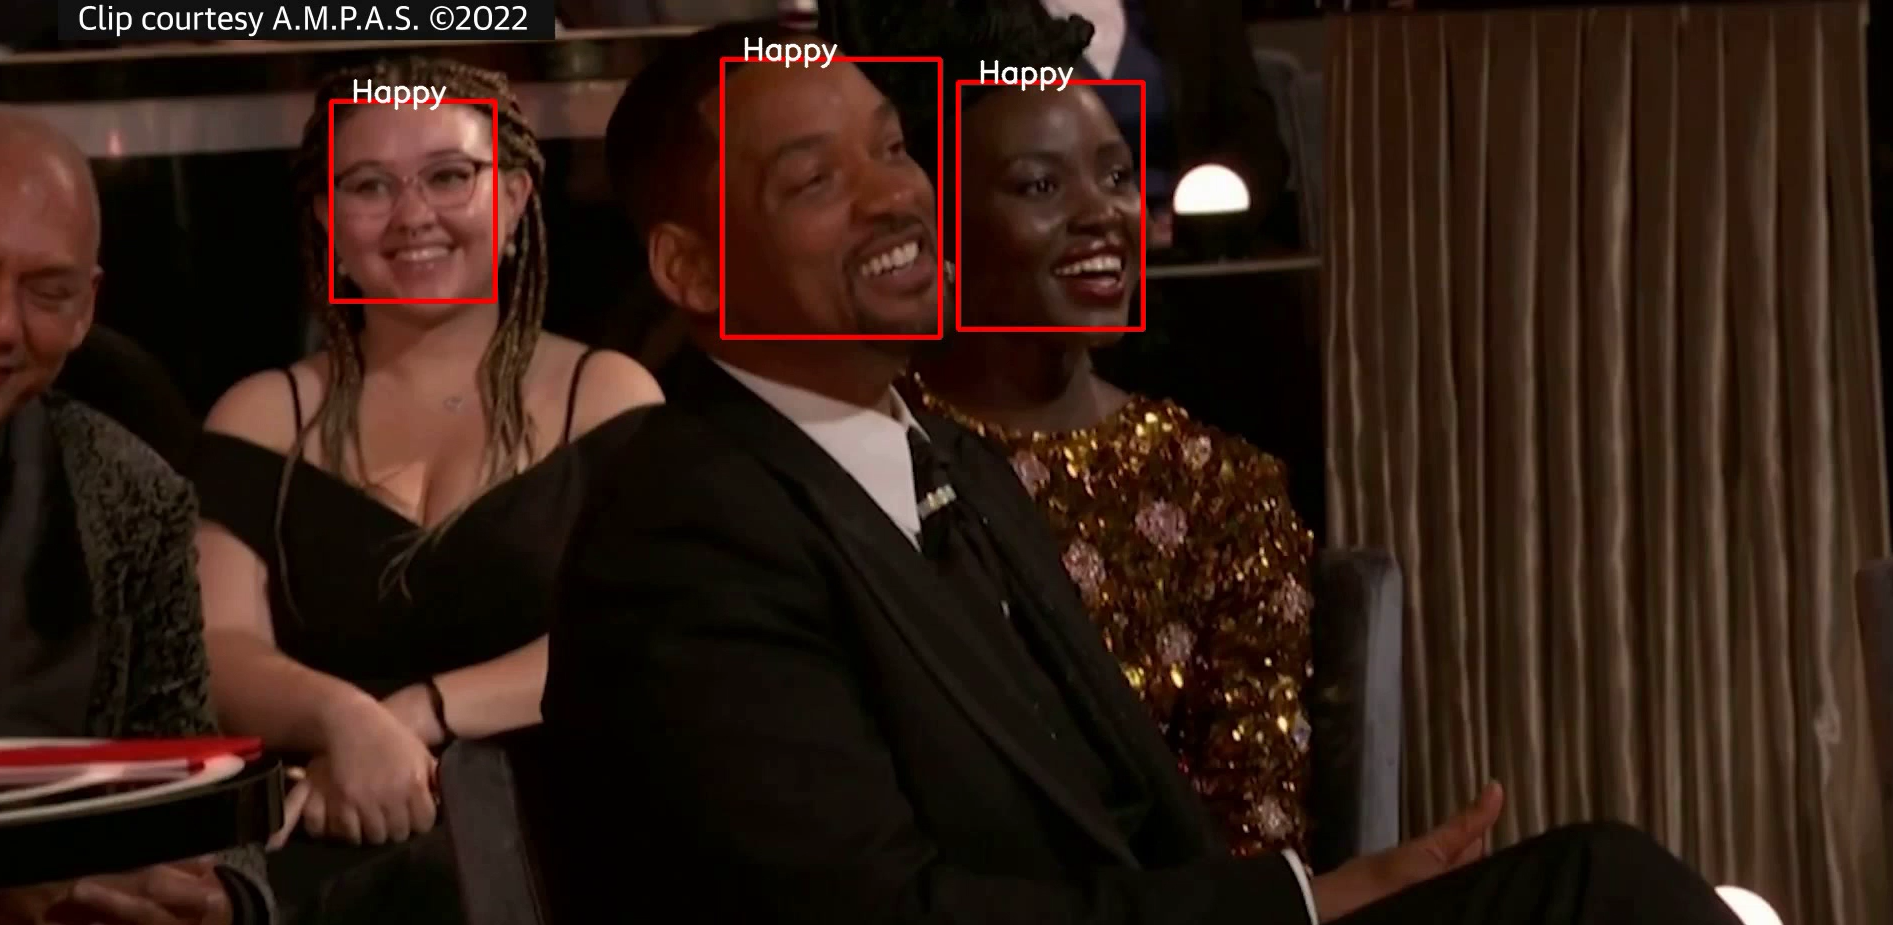
\includegraphics[width = 0.7\textwidth]{written_report/pictures/happy.png}
        \caption{Happy Faces}
        \label{fig:happy}
    \end{figure}
    \noindent
    \textbf{Implementation:} \texttt{emotion\_detection\textbackslash src\textbackslash video.py} \\
    \\
    % \subsubsection{Live Webcam}
    Back to our original objective of real time emotion detection, we use laptop webcam to capture real-time image, then pass it through into the model. The model runs pretty well in terms of performance, expect this demonstration is running on CPU, which results in very low frame rate.
    \begin{figure}[H]
        \centering
        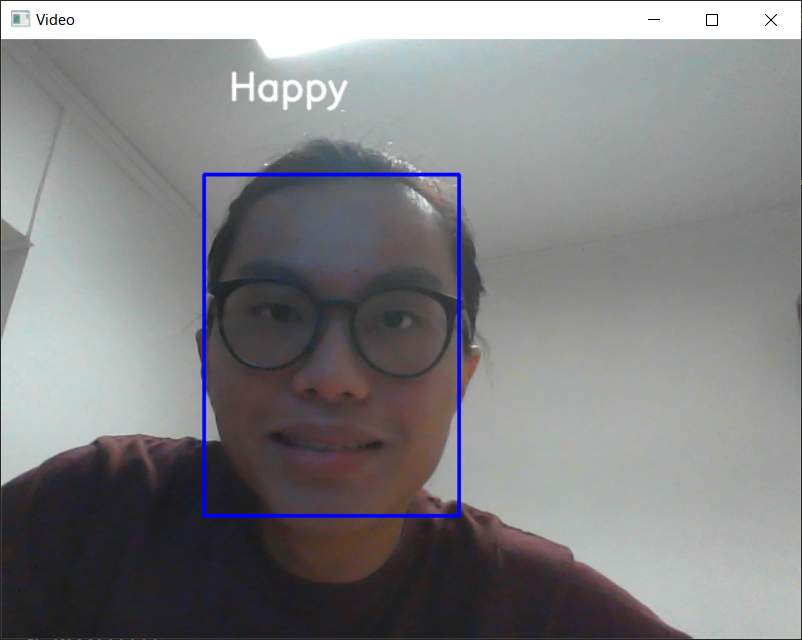
\includegraphics[width = 0.5\textwidth]{written_report/pictures/live_demo.png}
        \caption{Live Webcam Demonstration}
        \label{fig:live_webcam}
    \end{figure}
    \noindent
    \textbf{Implementation:} \texttt{emotion\_detection\textbackslash src\textbackslash real\_time\_webcam.py}
    
    \subsection{Discussion}
    \subsubsection{Basic Concept of Classification Evaluation}
    In this part, we will evaluate the performance of our CNN model by different indicators, namely confusion matrix, accuracy, precision, recall and F1-score. \\
    \\
    \textbf{Confusion matrix}: confusion matrix can show the summary of prediction and will be used to calculate accuracy, precision, recall and F1-score. 
    \begin{table}[H]
        \centering
        \begin{tabular}{c|c|c}
             & \multicolumn{2}{c}{\textbf{True Class}} \\
            \hline
            % \parbox[t]{2mm}{\multirow{2}{*}{\rotatebox[origin=c]{90}{Predicted Class}}}
            \multirow{2}{*}{\textbf{Predicted Class}} & True Positive (TP) & False Positive (FP) \\
            \cline{2-3}
             & False Negative (FN) & True Negative (TN)
        \end{tabular}
        \caption{Confusion Matrix}
        \label{tab:confusion_matrix}
    \end{table}
    \noindent
    Since our project is performing multi-class classification, an example of multi-class classification confusion matrix that an angry image is predicted as angry will be given as follows:
    \begin{table}[H]
        \centering
        \begin{tabular}{c|c|c|c|c|c|c|c|c}
             & & \multicolumn{7}{c}{\textbf{True Class}} \\
            \cline{3-9}
             & & Angry & Disgust & Fear & Happy & Neutral & Sad & Surprise \\
            \cline{2-9}
            \parbox[t]{2mm}{\multirow{7}{*}{\rotatebox[origin=c]{90}{\textbf{Predicted Class}}}} & Angry & TP & \multicolumn{6}{c}{FP} \\
            \cline{2-9}
             & Disgust & \multirow{6}{*}{FN} & \multicolumn{6}{c}{\multirow{6}{*}{TN}} \\ \cline{2-2}
             & Fear & \\ \cline{2-2}
             & Happy & \\ \cline{2-2}
             & Neutral & \\  \cline{2-2}
             & Sad & \\ \cline{2-2}
             & Surprise & 
        \end{tabular}
        \caption{Multi-Class Confusion Matrix}
        \label{tab:multi_class_confusion_matrix}
    \end{table}
    
    \subsubsection{Model Evaluation}
    \begin{table}[H]
        \centering
        \begin{tabular}{c|c|c|c|c|c|c|c|c|c}
             & & \multicolumn{7}{c}{\textbf{True Class}} \\ \cline{3-9}
             & & Angry & Disgust & Fear & Happy & Neutral & Sad & Surprise \\ \cline{2-10}
            \parbox[t]{2mm}{\multirow{7}{*}{\rotatebox[origin=c]{90}{\textbf{Predicted Class}}}} & Angry & 557  &       9  &      59  &      53  &     134  &     127  &      19 & 958 \\ \cline{2-10}
             & Disgust & 35  &      51  &       8  &       4  &       3  &      10  &       0 & 111 \\ \cline{2-10}
             & Fear & 143  &      11  &     293  &      46  &     184  &     260  &      87 & 1024 \\ \cline{2-10}
             & Happy & 45  &       2  &      19  &    1542  &      94  &      47  &      25 & 1774 \\ \cline{2-10}
             & Neutral & 63  &       4  &      21  &      76  &     888  &     169  &      12 & 1233 \\ \cline{2-10}
             & Sad & 136  &      12  &      72  &      51  &     317  &     647  &      12 & 1247 \\ \cline{2-10}
             & Surprise & 32  &       1  &      74  &      58  &      70  &      14  &     582 & 831 \\ \cline{2-10}
              & & 1011 & 90 & 546 & 1830 & 1690 & 1274 & 737 & 7178
        \end{tabular}
        \caption{Prediction Outcome}
        \label{tab:prediction_outcome}
    \end{table}
    
    \begin{table}[H]
        \centering
        \begin{tabular}{c|c|c|c|c|c|c|c}
             & Angry & Disgust & Fear & Happy & Neutral & Sad & Surprise \\ \hline \hline
            Accuracy & 0.8809 &  0.9862 &  0.8629 &  0.9276 &  0.8402 &  0.8291 &  0.9437 \\ \hline
            Precision & 0.5814 &  0.4595 &  0.2861 &  0.8692 &  0.7202 &  0.5188 &  0.7004 \\ \hline
            Recall & 0.5509 &  0.5667 &  0.5366 &  0.8426 &  0.5254 &  0.5078 &  0.7897 \\ \hline
            F1-score & 0.5658 &  0.5075 &  0.3732 &  0.8557 &  0.6076 &  0.5133 &  0.7423 \\
        \end{tabular}
        \caption{Accuracy, Precision, Recall and F1-score}
        \label{tab:score}
    \end{table}
    \noindent
    In terms of accuracy, each class has great performance with all over 82\% accuracy. However, only using accuracy could not truly evaluate the overall performance, thus, we take F1-score to access performance among different classes. Form the table above, we can see that the performance of class \textbf{Fear} is the worst while the performance of class \textbf{Happy} is the best. The performance different of them is relatively large 0.3732 vs 0.8557. The reason may be \textbf{Fear} faces have similar characteristic with \textbf{Angry}, \textbf{Sad} and \textbf{Surprise}, we can see in Table \ref{tab:prediction_outcome} that the mentioned three classes also have many samples mislabeled as \textbf{Fear}. In such case, the CNN model is not able to identify unique characteristics to differentiate those classes.
    
    \subsection{Conclusion}
    In this part of our project, we have developed a CNN model to perform facial recognition instantly. There are seven emotions can be classified, namely, angry, disgust, fear, happy, sad, surprise and neutral. The FER-2013 dataset is used which contain 28,709 examples in training set and 3,589 examples in testing set. After we train the model, around 60\% testing images can be correctly classified. There are some factors will affect the classification accuracy rate of the model, like the quality of the images, the resolution of the images in each emotion class, mislabeling in the dataset, etc. To improve the accuracy, we can relabel the dataset to avoid misleading result, which, however, is extremely time consuming. The other way to make some possible improvements is to try other models, like recurrent neural network (RNN) or use some advance techniques, like Cycle Generative Adversarial Network (Cycle GAN), VGG-Face model and residual neural network (resnet). \\
    \\
    Facial recognition is used in different area nowadays which bring a huge benefit to our society. One big usage is customer service. Facial recognition can allow to record the emotion of the customer. The company can provide more training to the staffs if a certain proportion of customers get bad emotions after the service. Facial recognition can also assist to interview candidate. The trained model can determine the emotion of candidate automatically and report to the human recruiters which can reduce the cost. Our group believe that facial recognition will be more commonly used in the future.

    
    \newpage
    \section{Cryptocurrencies Price Forecasting}
    \textbf{This section is contributed by KWOK Ho Hin (SID: 1155126159), TSOI Tung Sing (SID: 1155127274) and LO Chak Kin Steven (SID: 1155125491).}
    
    \subsection{Introduction}
    With the rapid advancement in Deep Learning, experts have been searching for applications of deep learning models in various industries, especially in Finance. Deep Learning models, particularly LSTM model, have been used extensively in developing quantitative trading strategies. Typically, researchers tries to use LSTM to predict stock prices, or implied volatility in the case of options. \\
    \\
    In this project, we aimed to incorporate LSTM model in a Crypto Pairs Trading Strategy. We first identified potential cointegrated pairs (token0, token1) and their respective hedge ratio ($\beta$). Then we tried to use LSTM to predict the spread of the pair (i.e. token0 – $\beta~\cdot$ token1) using only price data. A simple pair trading strategy can be designed by keeping track of the long-term mean ($\mu$) and setting a threshold ($e$) – we may buy the spread when it is below $\mu - e$ and sell it when it is above $\mu + e$. It is under the assumption that the cointegrated relationship between the two token will remain unchanged, hence the spread will be a stationary time series and will revert to its long-term mean mu.
    
    \subsection{Dataset}
    We have collected 10 months of minute-frequency data for 16 tokens with high market capitalization and trading volumes from \href{https://www.binance.com/en}{Binance} api. It includes candlesticks data, stored in OHLCV\footnote{OHLCV is an aggregated form of market data standing for Open, High, Low, Close and Volume.} format, aggregated in minute timeframe. 
    
    \begin{table}[H]
        \centering
        \begin{tabular}{|c|c|c|c|}
            \hline
            BTC & ETH & DOGE & BNB \\
            \hline
            XRP & TRX & ZIL & ADA \\
            \hline
            WAVES & ETC & LTC & MATIC \\
            \hline
            LINK & EOS & ATOM & XLM &
            \hline
        \end{tabular}
        \caption{Full List of Tokens}
        \label{tab:crypto_tokens}
    \end{table}
    
    \subsection{Data Pre-processing / Feature Engineering}
    Before getting into the model, we processed the data in the following ways:
    \begin{enumerate}
        \item Front-filling missing data (if there’s any)
        \item Compute log returns
        \item Generate addition features (RSI, EMA, rolling-STD of different window length) 
        \item Split the dataset into pre-data (for cointegration test, 1 month) and data (for training and testing, remaining 9 months)
    \end{enumerate}
    
    \subsection{Model Design}
    We adopt a three-step process for our complete model. The flow of our model is as follows:
    \begin{enumerate}
        \item 
            Use nearest-neighbour algorithm with a cross-sectional snapshot (the first observation in pre-data for all 16 tokens) to find the two nearest neighbours for each of the tokens.
        \item 
            Pair tokens up with their corresponding neighbours and conduct augmented Engle-Granger Two-Step Cointegration Test on each pair. Rank them in ascending order by the t-statistics.
        \item 
            Compute the spread and use a LSTM model in predicting the upcoming movement of the spread
    \end{enumerate}
    
    \subsubsection{Nearest Neighbour}
    To ease our computation, instead of looping through all the combination of pairs for the 16 tokens (total of $16 \times 15 ~/~ 2 = 120$ pairs) and conduct cointegration test one by one, we form potential pairs by matching them with their two nearest neighbours. By feeding in a cross-sectional snapshot of our data into the nearest-neighbour Algorithm, we identify 38 potential cointegrated pairs, which is less than a third of the original pairs.
    \begin{table}[H]
        \centering
        \begin{tabular}{|c|c|c|}
            \hline
            DOGE - ZIL & LINK - BNB & ADA - XRP \\
            \hline
            MATIC - BNB & ATOM - ZIL & LTC - DOGE &
            \hline
        \end{tabular}
        \caption{Example of the Pairs}
        \label{tab:crypto_pairs}
    \end{table}
    
    % ** In addition to the table, I will try to make a graph of the pairs with T-SNE **
    % But need some time to see see how it works
    
    \subsubsection{Cointegration Test}
    For each of the 38 potential pairs, we conduct an augmented Engle-Granger two step cointegration test which, by the name, consists of two steps.
    \begin{enumerate}
        \item Estimating the long-run equilibrium of the two series with OLS regression 
        \item Conduct a unit root test (Augmented Dicky Fuller Test) on the OLS residuals
    \end{enumerate}
    \\
    The null hypothesis of the test is that there is no cointegrating relationship while the alternative hypothesis suggests that there is cointegrating relationship between the two. We reject the null hypothesis at a 5\% significance level when the $p$-value is smaller than 0.05. \\
    \\
    There are a total of 13 pairs that we successfully reject the null hypothesis at 5\% significance level.
    \begin{table}[H]
        \centering
        \begin{tabular}{l|r}
            pairs & tstat \\
            \hline \hline
            [EOS, ZIL] & -5.388334 &
            [EOS, DOGE] & -5.311655 &
            [XRP, BNB] & -4.886678 &
            [XLM, ZIL] & -4.370721 &
            [LINK, BNB] & -4.352107 &
            [LTC, ZIL] & -4.210387 &
            [ADA, LINK] & -4.151885 &
            [DOGE, ZIL] & -4.104011 &
            [LTC, DOGE] & -3.956726 &
            [ADA, XRP] & -3.704049
        \end{tabular}
        \caption{Sorted in Ascending Order by t-statistics}
        \label{tab:crypto_tstat}
    \end{table}
    
    \subsubsection{LSTM}
    
    \subsection{Model Analytic}
    
    \subsubsection{Model Training}
    
    \subsubsection{Model Testing}
    
    \subsubsection{Comparsion with Baseline Model}
    % depends whether have time – use the exact same set of feature to fit into a baseline model like ARIMA
    
    \subsection{Backtesting}
    
    \subsection{Conclusion}
    
    \newpage
    % \thispagestyle{empty}
    % \pagenumbering{gobble} 
    \section{Bibliography}
    \bibliographystyle{unsrt}
    % \bibliographystyle{plain} % We choose the "plain" reference style
    \bibliography{refs} % Entries are in the refs.bib file
    
\end{document}